\section{Dynamic Screening and UOT problem}
\subsection{Screening for UOT}

We can get the dual form of UOT problem: 
\begin{lem}
For $d(\X \vt) = \frac{1}{2}\|\X \vt-\y\|_2^2$, the dual Lasso problem has the following form:
$$
\begin{aligned}
d^*(-\theta) = \frac{1}{2}\|\theta\|_2^2-\y^{\tranT}\theta
\end{aligned}
$$

$$
g^*(\X^{\tranT}\theta) = \left\{
\begin{aligned}
0 \quad&\quad ( \forall \vt \quad\theta^{\tranT}\X\vt - g(\vt) \leq 0 )\\
\infty \quad&( \exists t \quad\theta^{\tranT}\X\vt - g(\vt) \leq 0 )
\end{aligned}
\right.
$$
\end{lem}


For UOT problem \ref{eq:uot}, we could get its dual form. 
\begin{lem}(Dual form of UOT problem)
\begin{equation}
\begin{split}
-d^*(-\theta) - g^*(\X^{\tranT}\theta)& = -\frac{1}{2}\|\theta\|_2^2-\y^{\tranT}\theta \\
 \mathbf{s.t.} \quad \forall i \quad \x_i^{\tranT}\theta -\lambda \vc_i &\leq 0
 \end{split}
 \label{eq:uotdual}
\end{equation}
\end{lem}
$\x_i $ is the i-th column of $\X$, these inequations \ref{eq:uotdual} make up a dual feasible area written as $\mathcal{R}^{D}$, and the optimal solution definitely satisfied them.\\
From the KKT condition, we konw that, for the optimal primal solution $\hat{\vt}$:
\begin{thm} (KKT condition) For the dual optimal solution $\hat{\theta}$, we have the following relationship:
 \begin{equation}
\begin{split}
\x_i^{\tranT}\hat{\theta} -\lambda \vc_i  \left\{
\begin{aligned}
< 0 \quad& \Rightarrow \hat{\vt}_i = 0\\
= 0 \quad& \Rightarrow \hat{\vt}_i \geq 0
\end{aligned}
\right.
 \end{split}
 \label{eq:kkt}
\end{equation}
\end{thm}

As we do not know the information of $\hat{\vt}$ directly, we can construct an area $\mathcal{R}^{S}$ containing the $\hat{\vt}$, if

\begin{equation}
\max_{\vt \in \mathcal{R}^S} \x_i^{\tranT}\theta -\lambda \vc_i  < 0
\end{equation}
then we have:
 \begin{equation}
 \x_i^{\tranT}\hat{\theta} -\lambda \vc_i  < 0
\end{equation}
which means the corresponding $\hat{t}_i = 0$, and can be screening out.

Before we start to construct the area containing $\hat{\theta}$, from \ref{circle} we know that, we have to find a $\tilde{\theta}$ in the dual feasible area before we construct any area, there is a relationship between the primal variable and dual variable $\theta = \y - \X\vt$, however, the outcome $\theta$ might not inside the dual feasible area, which encourage us to project. In lasso problem, as the constraints limit the$\|\x_i \theta\|_1$,  researchers would use a shrinking method like: 
\begin{equation}
\tilde{\theta} = \frac{(\y - \X \vt)}{\max(\lambda \vc, \|\X^{\tranT}(\y-\X\vt)\|_{\infty})}
\end{equation}
Then $\tilde{\theta}$ would be in the dual feasible are. As for UOT problem, it only allow $\vt_i \geq 0$, and its $x_i$ only consists of two non-zero elements, which allows us to adapt a better projection method:


\begin{thm}
(UOT projection) For any any $\theta \in \R^{n+m}$, we can compute the projection $\tilde{\theta}$ onto the dual feasible area, $j_1$ and $j_2$ indicates the non-zero elements in each $x_j$
 \begin{equation}
		\tilde{\theta}_{i}=\left\{
	\begin{aligned}
			&\theta_{i} - \max_{j \mid n = i}(\frac{\theta_{j_{1}}+\theta_{j_{2}}-\vc_j}{2}) & 0\leq i<m\\
			&\theta_{i} - \max_{j \operatorname{mod} n= i-m}(\frac{\theta_{j_{1}}+\theta_{j_{2}}-\vc_j}{2}) & m\leq i<n+m
	\end{aligned}
	\right.
 \end{equation}
\end{thm}
	\begin{figure}[htbp]
	\begin{center}	
	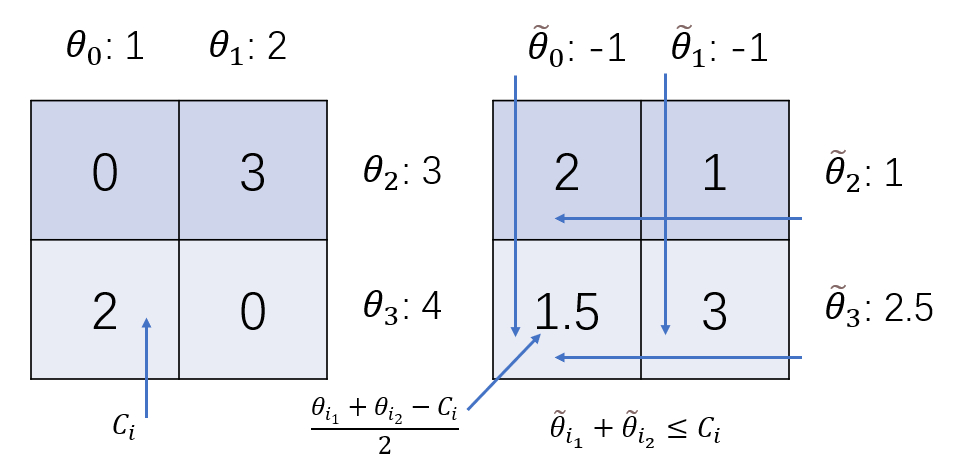
\includegraphics[width=0.8\hsize]{pic/shifting}
	\caption{Shifting on a 2$\times$2 matrix}
	\end{center}	
	\end{figure}

As we have got the $\tilde{\theta}$ in the $R^{D}$ and we also have another constraint area $\mathcal{R}^{C}$, we are sure that the $\hat{\vt} \in \mathcal{R}^{C}\cap\mathcal{R}^{D}$. However, The intersection of a sphere and a polytope can not be compute in $O(knm)$, where $k$ is a constant.  We design a relaxation method. which divide the constrains into two parts, then we are maximizing on the intersection of two hyperplanes and a hyper-ball. 

\begin{thm}\label{area}(Screening Area for UOT) With the help of $\tilde{\theta}$, we can construct following area $\mathcal{R}^{S}$, and the optimal dual solution $\hat{\theta}$ must be inside the area.
 \begin{equation}
\begin{split} 
\mathcal{R}^S = \{ \theta \|
\begin{aligned}
 &\theta^{\tranT}\X^A\beta - \lambda g^{A}\beta\leq 0 \\
  &\theta^{\tranT}\X^B\beta - \lambda g^{B}\beta \leq 0\\
   &(\theta-\tilde{\theta})^{\tranT}(\theta-\y)\leq 0\}
\end{aligned}
\end{split}
\label{eq:divide}
\end{equation}
\end{thm}
We devide the constraints into two group $A$ and $B$, we have $\X^A +\X^B=X$ and $g^A+g^B = g$
the computational process is in Appendix.A

\subsection{Screening Algorithms}

 \begin{algorithm}
 \caption{UOT Dynamic Screening Algorithm}
 \begin{algorithmic}[1]
 \renewcommand{\algorithmicrequire}{\textbf{Input:}}
 \renewcommand{\algorithmicensure}{\textbf{Output:}}
 \REQUIRE $t_0, S \in R^{n\times m}, S_{ij}=1$
 \ENSURE  $S$
  \STATE \text{Choose a solver for the problem.}
  \FOR {$t = 0 \text{ to } K$}
  \STATE $\text{Projection } \tilde{\theta} = \operatorname{Proj}(t^k)$ 
  \IF {($i \ne 0$)}
  \STATE $\textbf{break}$
  \ENDIF
    \STATE $\mathcal{R} \Leftarrow \mathcal{R}^S{(\tilde{\theta},t^k)}$
    \STATE $S \Leftarrow {S_{ij} = 0 \text{ if } \max_{\theta \in \mathcal{R}^S} {x_{k(i,j)}}^{\tranT}\theta <\lambda c_{k(i,j)} }$
    \FOR {$a  \in {A_{ij}\|A_{ij}=0}$}
    \STATE $t^k(i,j) \Leftarrow 0$
    \ENDFOR
    \STATE $t^{k+1} = \operatorname{update}(t^k)$
  \ENDFOR
  
 \RETURN $t^{K+1}, S $ 
 \end{algorithmic} 
 \end{algorithm}

screening method is irrelevent to the optimization solver you choose. We give the specific algorithm for $L_2$ UOT problem to show the whole optimization process.\\











































